\experiment{Construcción del Montaje}

Para la construcción de los péndulos físicos, se utilizaron barras
metálicas obtenidas en el taller de máquinas y herramientas de la
sede Macarena, las cuales cumplían con el requisito previamente
planteado de emplear un material con alta densidad.
Del mismo modo, se avanzó en la preparación del sistema de medición
de ángulos mediante el sensor \emph{Cassy}, revisando su funcionamiento,
calibración y evaluando la forma de integrarlo al sistema.
Para finalizar, se llevó a cabo la medición de la constante
elástica de los resortes inicialmente seleccionados para la
práctica. Estos resortes fueron adquiridos en una fábrica
especializada con el fin de garantizar constantes elásticas
nominales similares y condiciones físicas consistentes.

\subexperiment{Construcción de los péndulos}
En el taller se identificó una varilla metálica de sección
adecuada. Esta varilla presentaba la rigidez necesaria para
nuestro experimento, por lo que se decidió utilizarla.
A partir de ella, se cortaron las barras con las longitudes
especificadas para el sistema (\(l\) para el central y \(l/2\)
para los laterales). Posteriormente, se pulieron los bordes
para evitar imperfecciones o filos peligrosos, y se perforaron
los orificios necesarios para su montaje.
En el caso de las barras de longitud \(l/2 = \qty{28.0(1)}{\centi\metre}\),
los orificios se realizaron a una distancia de \qty{4.6(1)}{\centi\metre}
desde cada extremo.

Adicionalmente, se midieron las masas de las barras y se determinó
la posición de sus respectivos centros de masa,
medidos desde el punto de pivote. Los resultados se resumen en la
\cref{tab:bars-dat}.

\pgfplotstableread[col sep=comma, header=true]{
	i, y_cm_i, m_i
	1, 14.2, 0600.8
	2, 28.0, 1216.3
	3, 14.0, 0601.8
}\mydata

\begin{table}[htbp!]
	\centering
	\pgfplotstabletypeset[
	col sep=comma,
	zerofill,
	columns/i/.style={
		string type,
		column type={c},
		column name={\(i\)},
	},
	columns/y_cm_i/.style={
		column name={\(y_{\text{cm}_i} [\si{\centi\metre}]\)},
		precision=1,
		fixed,
		fixed zerofill,
	},
	columns/m_i/.style={
		column type={c},
		column name={\(m_i [\si{\gram}]\)},
		dec sep align,
		precision=1,
		fixed,
		fixed zerofill,
	},
	every head row/.style={
		before row=\toprule,
		after row=\midrule,
	},
	every last row/.style={
		after row=\bottomrule,
	}
	]\mydata
	\caption{Parámetros físicos de las barras empleadas en el montaje.
		La incertidumbre para la posición del centro de masa (\(y_{\text{cm}_i}\))
		es de \qty{0.1}{\centi\metre} y para la masa (\(m_i\)) es de
	\qty{0.1}{\gram}.}
	\label{tab:bars-dat}
\end{table}

\begin{figure}[htbp!]
	\centering
	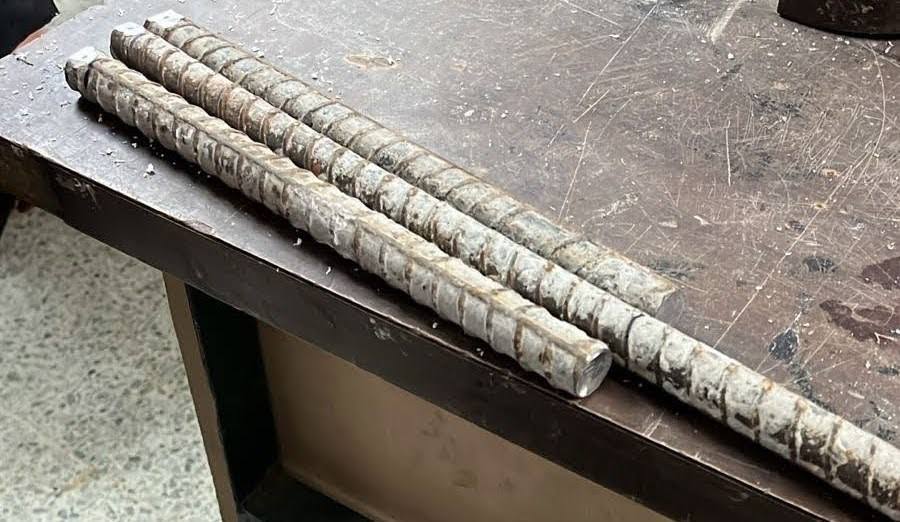
\includegraphics[width=0.7\linewidth]{./Figures/metal-bars.jpeg}
	\caption{Barras metálicas preparadas para el montaje de los péndulos.}
	\label{fig:metal-bars}
\end{figure}

\subexperiment{Preparación del Dispositivo \emph{Cassy}}
Se realizó una revisión inicial del sistema de medición \emph{Cassy}.
Esta observación permitió definir una estrategia preliminar para
su integración en el sistema, con el fin de registrar los
ángulos de oscilación. Se empleará alambre dulce para fijar las
barras a la rueda giratoria de cada sensor, utilizando los
orificios correspondientes en ambas partes.

\subexperiment{Medición de la constante elástica}
Se llevó a cabo la medición de la constante elástica de los
resortes que se planea utilizar en el experimento. Para esto,
se empleó el montaje experimental convencional de aplicar masas
conocidas a cada resorte, medir su elongación y, mediante una
regresión lineal de desplazamiento en función de la masa soportada,
estimar su constante de elasticidad.

Se utilizaron masas en un rango de \qty{50}{\gram} a \qty{80}{\gram}.
Para dos resortes representativos, se obtuvieron constantes de
elasticidad de \(k_1 = \qty{3.04(4)}{\N\per\m}\) y
\(k_2 = \qty{3.32(6)}{\N\per\m}\). Los valores de desplazamiento
según la masa aplicada se presentan en la \cref{fig:springs-plot}.

\begin{figure}[htbp!]
	\centering
	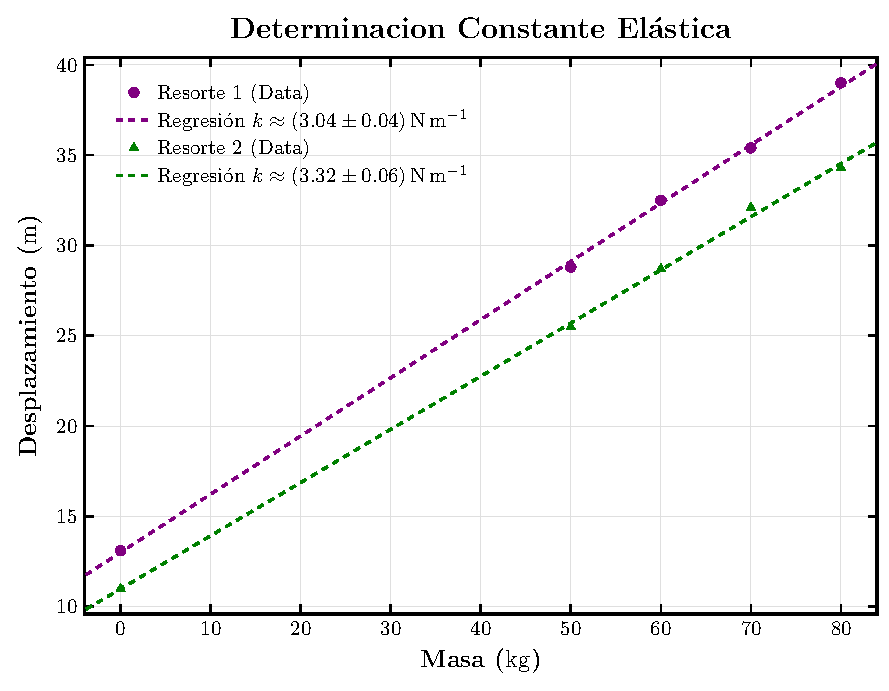
\includegraphics[width=0.6\linewidth]{./Figures/springs-plot.pdf}
	\caption{Determinación de la constante elástica de los resortes.}
	\label{fig:springs-plot}
\end{figure}
